We trained a Tree-Augmented Naïve Bayes network on 20,950 training cases and measured the incompleteness score on 3,695 test cases, results are shown in figure \ref{fig:incompleteness_score_hist_all}. The resulting incompleteness scores were heavily right-skewed distributions. 83\% of the incompleteness scores were equal to zero, meaning no new information would have changed the follow-up decision. Hence, both the median and mode incompleteness scores were zero. The mean incompleteness score was 0.021.

\begin{figure}[h!]
\centering
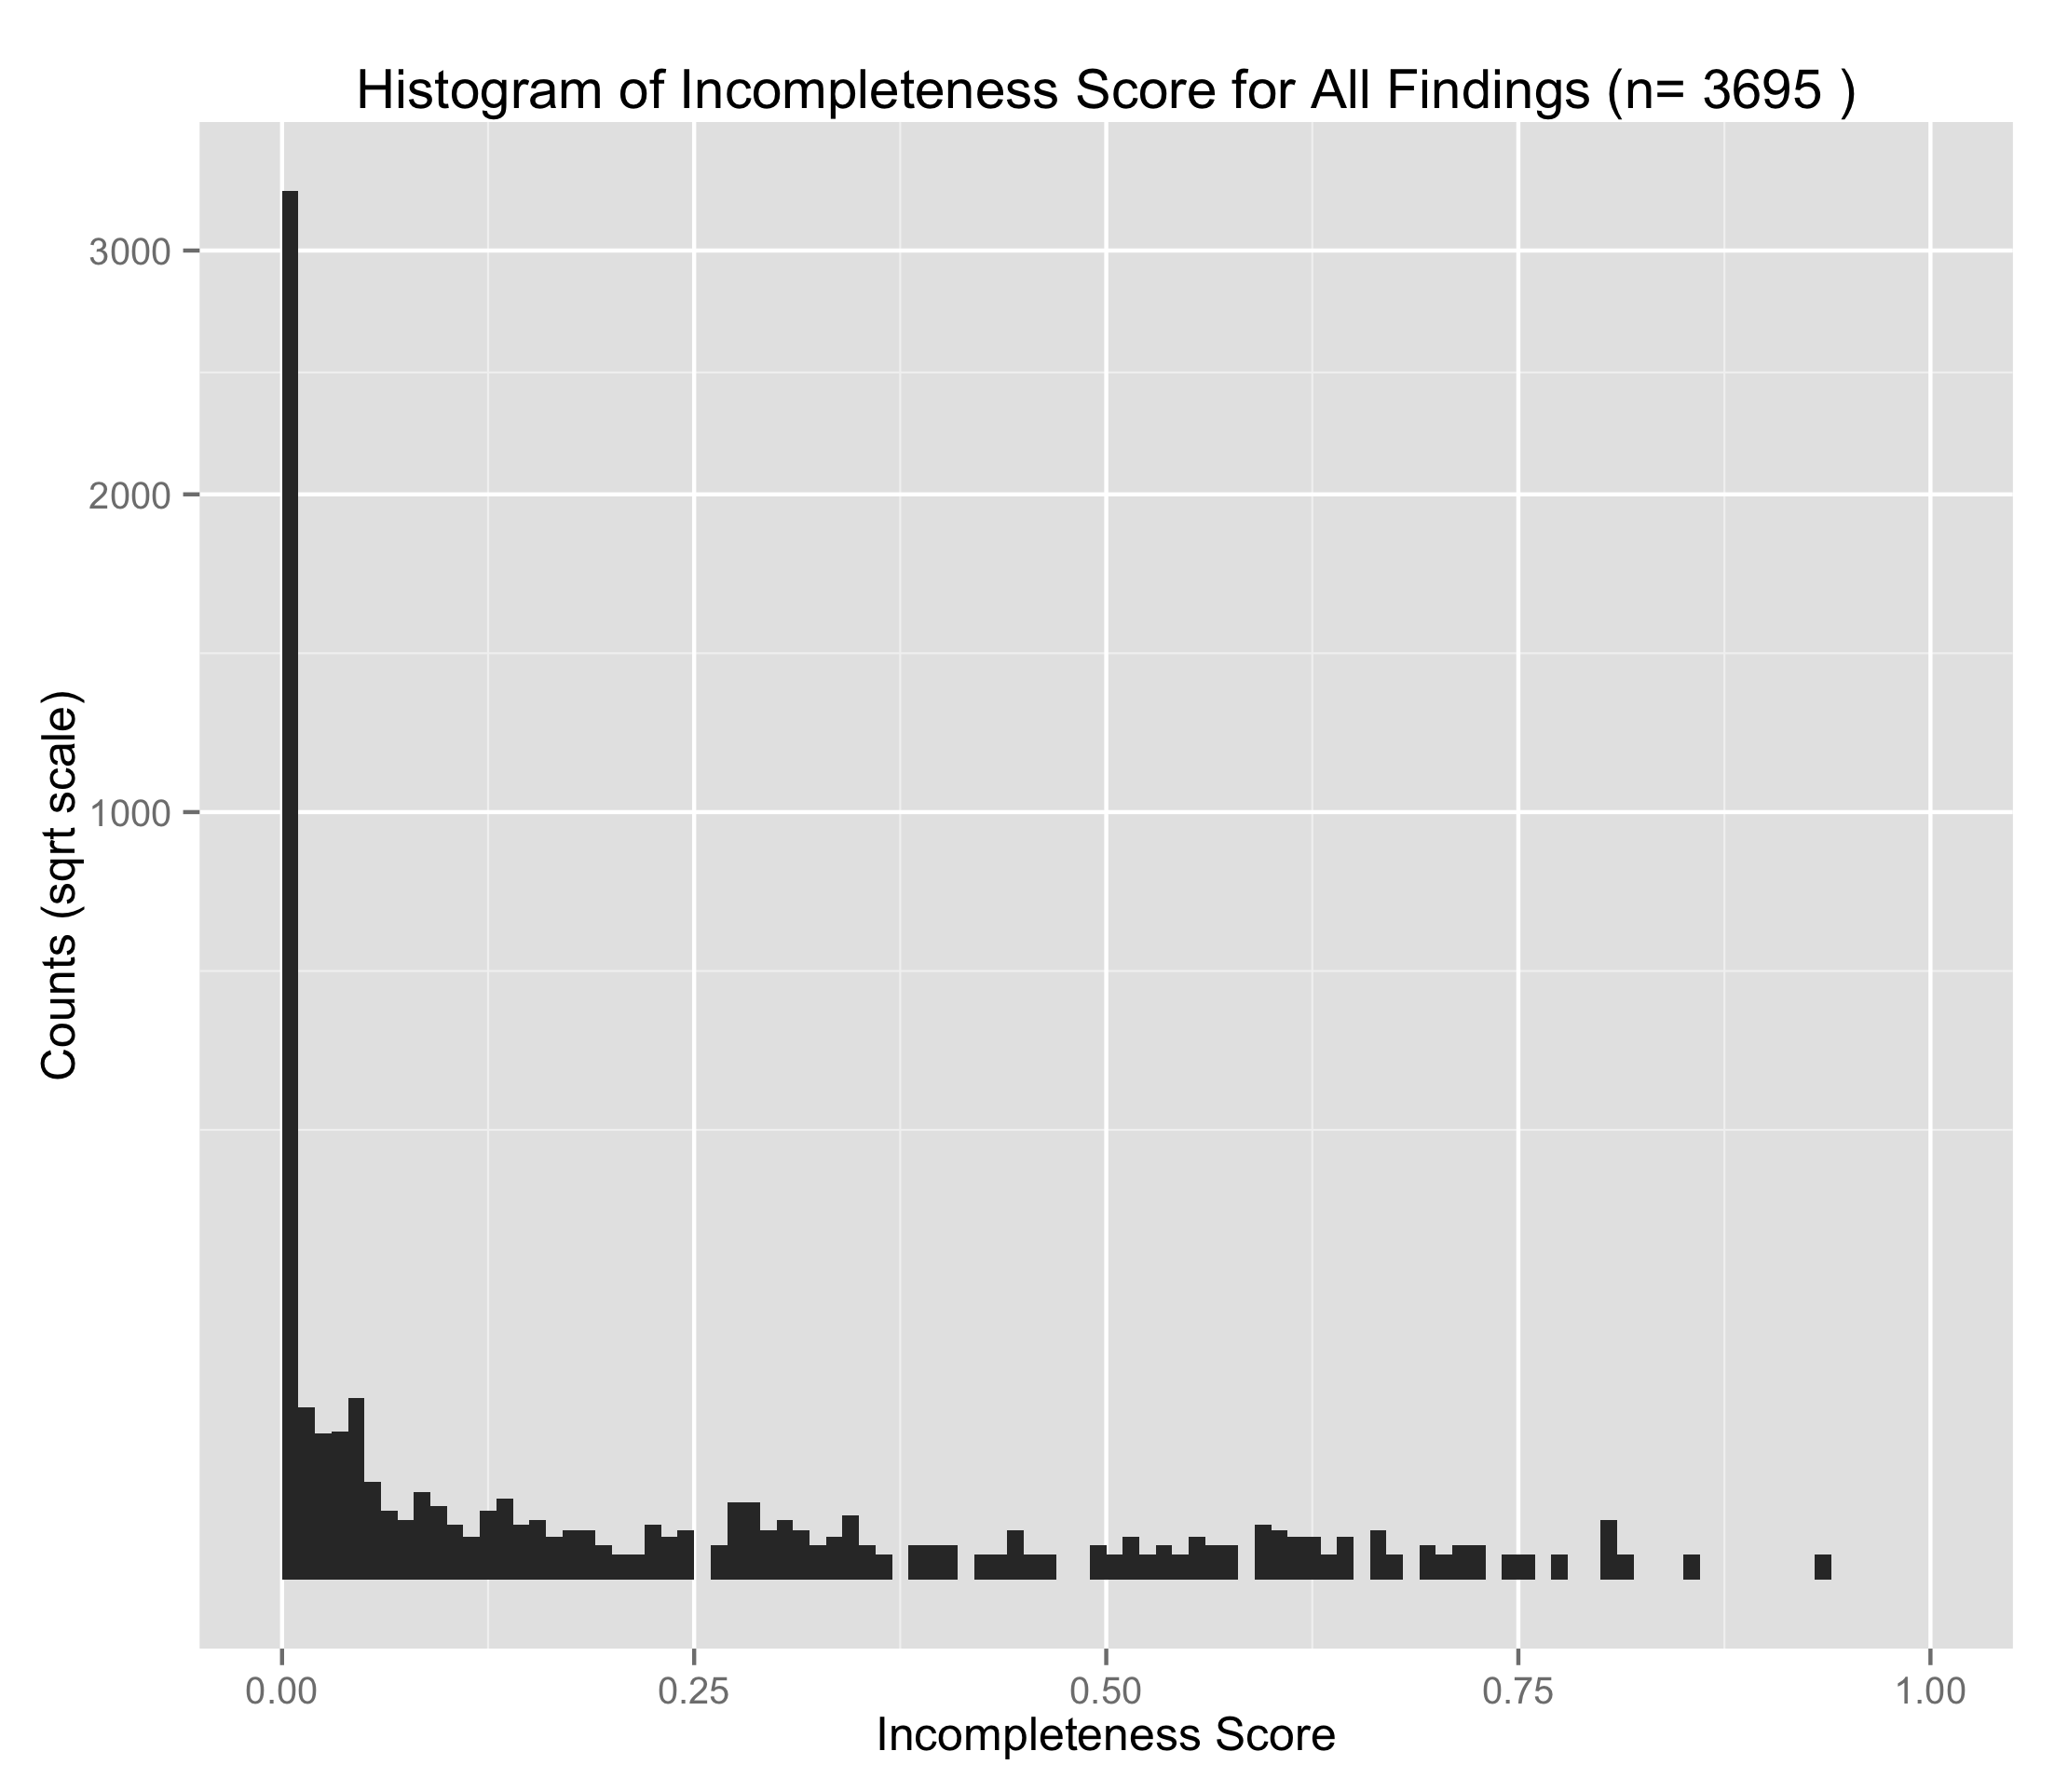
\includegraphics[width=\linewidth]{figures/incompleteness_score_hist_all}
\caption{Histogram of all incompleteness scores in the test data set}
\label{fig:incompleteness_score_hist_all}
\end{figure}


In order to verify that the incompleteness score can be used to predict mammographic error, we plotted its histogram and density estimate stratified by radiological predictive categories: true negative (TN), false negative (FN), true positive (TP), and false positive (FP) [Figure 1]. The graphs show that there are a large number of false positive and false negative cases that have non-zero incompleteness scores. Intuitively, this shows that incomplete reports have a higher likelihood of containing errors. The difference between error (FP,FN) and non-error (TP,TN) incompleteness scores was statistically significant (p < 2.2*10-16). 

An issue with this data is that there are a small number of false negative findings compared to false positive findings. This could skew results since positive findings may contain descriptors more prone to noise in the model. To account for this, we compared false positive to true positive results since both groups would have similar descriptors. The analysis showed that they were still statistically significantly different (p<0.0026).

We then tested how well the incompleteness score could predict error in mammography reading. Figure 2 shows several performance metrics for different cutoffs of the incompleteness score. The maximal accuracy with respect to cutoffs was 0.826 at a cutoff of 0.018. This means that > 1.8\% probability of changing decisions when given new information should warrant describing more observations. The precision associated with this cutoff was 0.713 meaning 71.3\% of cases classified as errors via the incompleteness score with cutoff 0.018 will actually be errors. Finally, we measured the percentage reduction in total mammography error if each error marked for revision was corrected. Using the given cutoff, we saw a potential 21.7\% decrease in total errors.
